\section{Held-out calibration of the browser linear forecast}
\label{sec:browser-calibration}

The browser forecast is a global linear map fitted to synthetic windows, not
the locally trained neural implementation that shares the NLinear name in the
offline comparison. This distinction matters because a name does not identify
a loss function, a training sample or an uncertainty procedure. The original
browser matrix has 48 input coordinates and 12 output coordinates. It is
estimated by least squares on 52,144 overlapping windows drawn from 400
generated series. Its point forecasts run through an actual ONNX matrix
multiplication in the browser. Neither this small representation nor its
execution speed establishes that its forecast distribution is calibrated.

In the previous implementation, a pooled training-residual standard deviation
was multiplied by the observed window's scale and by the square root of the
forecast lead. This rule produces finite bands, but no held-out experiment had
established their nominal coverage. Training residuals reuse outcomes that
helped estimate the map; pooling leads also discards the error distribution's
dependence on forecast distance. Multiplying that pooled scale by another
lead-dependent factor is an engineering approximation rather than a consequence
of the fitted global regression. The following experiments evaluate that
specific implemented rule. They do not treat Gaussian intervals as a uniformly
weak baseline or extrapolate their behavior to every model with Gaussian errors.

The first experiment tested a fixed regularization grid and independent
calibration. Its point-error result was unfavorable. A second, separately
specified experiment therefore retained the original point matrix and tested
prefix-stratified interval calibration on fresh generated series. This sequence
separates an observed failure from a new confirmation. It does not permit the
first test set to become the second experiment's tuning set while still being
described as independent confirmation. The complete first result remains in
the record, including its validation decision and family-specific coverage.

\subsection{Observed-window normalization and a fixed point map}
\label{sec:browser-normalization}

Let $x=(x_1,\ldots,x_L)$ be the last $L=48$ observations and let $a_h$ denote
the target at lead $h\in\{1,\ldots,12\}$. All normalization quantities are
computed from $x$, before any target is revealed. Define
\begin{equation}
 \bar x=L^{-1}\sum_{i=1}^L x_i,\qquad
 s(x)=\left[L^{-1}\sum_{i=1}^L(x_i-\bar x)^2\right]^{1/2},\qquad
 z_i=\frac{x_i-x_L}{s(x)}.
 \label{eq:browser-normalization}
\end{equation}
For a matrix $W\in\mathbb R^{L\times H}$, the normalized prediction is
$\hat u=z^\top W$ and the prediction in the observation's units is
\begin{equation}
 \hat a_h=x_L+s(x)\hat u_h.
 \label{eq:browser-inverse}
\end{equation}
The matrix contains no intercept. Subtraction of the last observation fixes the
origin used by the exported model; subtraction of the sample mean would define
a different predictor. The denominator is the population standard deviation of
the observed window, not the residual standard deviation of a trend fit. The
training recipe and browser implementation use this same convention.

If $s(x)=0$, the normalized model is unavailable. Substituting a raw-unit scale
of one would change the computation when the same constant sequence is expressed
in different units. A constant sequence can be forecast by a separately declared
constant predictor, but that is not evidence for assigning a calibrated
uncertainty scale to this normalized map. Nonfinite observations, unsupported
horizons and malformed matrix outputs are also refused. The 12-lead model does
not generate additional leads by repeating its last output.

The deployed matrix is preserved byte-for-byte throughout both experiments.
Its SHA-256 is recorded with the calibration metadata, and the browser verifies
the actual downloaded graph against that digest before inference. This prevents
a valid calibration array from being accidentally paired with a different
point map. Numerical parity is checked independently using the float32 graph
and a NumPy multiplication. Agreement of those computations is a numerical
identity check; it is not a forecasting-performance claim.

\subsection{Regularization, selection and the first held-out experiment}
\label{sec:browser-ridge}

The training collection uses the original generator and random sequence. Each
series is assigned one of four equally probable mechanisms: sinusoidal
seasonality, trend plus seasonality, trend, or independent noise. Periods are
selected from six, twelve and twenty-four observations; series lengths are
sampled from the integer interval $[120,260)$. These are controlled mechanisms,
not observations from the electricity, air-quality or competition datasets.
The overlapping windows within one training series share observations. They
therefore cannot be used as independent calibration or test replications.

For normalized training rows $Z$ and targets $U$, the candidate family minimizes
\begin{equation}
 \widehat W_\lambda=\mathop{\rm argmin}_{W}
 \left\{\frac{1}{N}\|U-ZW\|_F^2+\lambda\|W\|_F^2\right\}.
 \label{eq:browser-ridge}
\end{equation}
The fixed grid is $\{0,10^{-6},10^{-4},10^{-2},10^{-1},1,10\}$. The zero entry
uses a least-squares solver, including when the Gram matrix is singular.
Positive penalties solve the regularized normal equations. Candidate matrices
are converted to float32 before validation. Selection minimizes mean normalized
squared error on the final complete window of each of 200 independent
validation series. Exact ties select the earlier grid entry. The selected
matrix is not refitted using the validation or calibration series.

Four hundred additional series supply calibration errors and another four
hundred supply test errors. A series contributes only its final complete
48-to-12 window outside training. The training, validation, calibration and test
generators use local PCG64 seeds 20260704, 20261105, 20261106 and 20261107,
respectively. These integers identify generator streams; they are not dates of
data collection. Full-sequence hashes verify that no series is duplicated
across any partition. Family labels are retained for evaluation, but do not
enter the fitted linear map.

Validation selected $\lambda=0.1$. On the independent test sample, normalized
mean squared error was 0.550561, compared with 0.548742 for the frozen original
map. The paired difference was $+0.001819$, with an exploratory 95\% series
bootstrap interval $[0.000145,0.003465]$. Only 150 of 400 series had lower
squared loss. Thus the validation-selected ridge candidate did not improve the
point forecast in this experiment. This outcome is retained rather than
replaced by the favorable validation score or a new penalty chosen from test
outcomes. A repeat-last control had normalized squared error 1.795089, which
locates both linear maps relative to a simpler forecast without making either
map an unconditional winner outside this generator.

\subsection{Per-lead split calibration and its conditional limits}
\label{sec:browser-split}

For a fixed point model and independent calibration series indexed by $j$,
define the absolute normalized error at lead $h$ as
\begin{equation}
 R_{jh}=\left|\frac{a_{jh}-\hat a_{jh}}{s(x_j)}\right|.
 \label{eq:browser-residual}
\end{equation}
With $n$ calibration series and miscoverage $\alpha=0.2$, the radius is the
$k$th order statistic,
\begin{equation}
 k=\lceil(n+1)(1-\alpha)\rceil,\qquad
 q_h=R_{(k)h},\qquad
 I_h(x)=[\hat a_h-s(x)q_h,\hat a_h+s(x)q_h].
 \label{eq:browser-radius}
\end{equation}
If $k>n$, a finite empirical radius is not available under this convention.
Interpolation of the nominal 80th percentile is not substituted for the
specified finite-sample rank. For $n=400$, the selected one-based rank is 321.
Calibration uses the actual runtime output of the exported point model, so
calibration and testing apply the same numerical predictor.

For independent exchangeable calibration and test series and a point model
fixed before calibration, the rank of the new residual among the $n+1$
residuals is uniform in the absence of ties; conservative tie handling gives
the usual lower coverage bound. Consequently
\begin{equation}
 \Pr\{a_h\in I_h(x)\}\geq 1-\alpha.
 \label{eq:browser-marginal-guarantee}
\end{equation}
This is a marginal statement over new series from the same population,
separately for each lead~\cite{splitintro}. It does not say that all twelve
future observations are covered together with probability 0.8. Nor does it
guarantee 0.8 conditional coverage for each observed prefix, each latent
generator family or an arbitrary authentic series. Internal serial dependence
within one generated series does not by itself invalidate exchangeability
across independently generated series; pooling dependent windows as separate
calibration observations would be a different design.

In the first test sample, the calibrated ridge intervals had 79.46\% overall
coverage, normalized mean width 1.659786 and normalized interval score 2.781262.
The original Gaussian rule had 96.60\% coverage, width 4.593046 and score
4.764406. However, the calibrated candidate's white-noise coverage was only
53.06\%, while seasonal and trend-plus-seasonal coverage exceeded 93\%.
The aggregate result therefore could not support a statement that all
mechanisms were calibrated. It motivated a new prefix-stratified procedure
and a fresh confirmation population, while leaving the original result intact.

\subsection{Prefix-roughness strata and independent confirmation}
\label{sec:browser-strata}

The second experiment changes intervals while preserving exactly the original
point predictions. Its observable grouping statistic is
\begin{equation}
 \rho(x)=\frac{(L-1)^{-1}\sum_{i=1}^{L-1}(x_{i+1}-x_i)^2}
 {L^{-1}\sum_{i=1}^L(x_i-\bar x)^2}.
 \label{eq:browser-roughness}
\end{equation}
The three fixed bins are $[0,0.5)$, $[0.5,1.25)$ and $[1.25,\infty)$.
This ratio compares local changes with total observed variation. Independent
noise has population ratio near two; a well-sampled sinusoid has ratio
approximately $2\{1-\cos(2\pi/m)\}$. These relationships motivate separating
smooth, oscillatory and rough prefixes without using a hidden mechanism label.
The boundaries are engineering choices fixed before the new confirmation
outcomes, rather than estimated cut points optimized on those outcomes.

For a bin $b$, the calibration radius uses only series whose observed prefixes
belong to $b$:
\begin{equation}
 q_{bh}=R_{(k_b)h}^{(b)},\qquad
 k_b=\lceil(n_b+1)(1-\alpha)\rceil.
 \label{eq:browser-group-radius}
\end{equation}
At least twenty independent calibration series are required in every bin.
Conditional on a fixed prefix partition and exchangeable series within a bin,
the rank argument applies separately in that bin. It does not acquire validity
within every latent family simply because the bin was computed from a prefix.
The number of calibration series per bin affects the granularity and sampling
variability of each radius; finer partitions can therefore reduce efficiency
or leave a bin without an admissible radius.

The confirmation uses 400 new calibration series from seed 20261109 and 800
new test series from seed 20261110. Their full-sequence hashes are disjoint
from all 1,400 series in the first experiment. The point map is not trained,
selected or updated in this confirmation. Its Gaussian, globally calibrated
and prefix-stratified interval arms use identical points at every test origin.
Calibration bin counts were 115, 120 and 165. This yields finite-sample ranks
93, 97 and 133, respectively. The global arm uses all 400 calibration series
and provides a matching ablation of the prefix partition.

\begin{algorithm}[htbp]
\caption{Fixed-point forecast with prefix-stratified marginal intervals. Every
quantity used at prediction time is determined before observing the next target.}
\label{alg:browser-calibration}
\begin{algorithmic}[1]
\Require Frozen point matrix $W$, independently calibrated radii $q_{bh}$,
observed prefix $x$, supported horizon $H=12$
\State Refuse nonfinite observations, an incomplete lookback or $s(x)\leq0$
\State Compute $z$ from Equation~\ref{eq:browser-normalization}
\State Select the fixed bin $b$ containing $\rho(x)$
\State Compute $\hat u=z^\top W$ using the verified float32 ONNX graph
\For{$h=1,\ldots,H$}
\State Set $\hat a_h=x_L+s(x)\hat u_h$
\State Store $I_h=[\hat a_h-s(x)q_{bh},\hat a_h+s(x)q_{bh}]$
\EndFor
\State \textbf{return} $(I_1,\ldots,I_H)$
\end{algorithmic}
\end{algorithm}

Algorithm~\ref{alg:browser-calibration} requires $O(LH+L)$ arithmetic after
the small fixed graph has been loaded. It carries no recurrent hidden state
and performs no online refit. Hash verification binds the graph to the radii;
it does not identify whether a new series belongs to the calibration
population. The browser therefore describes the intervals as nominal marginal
bands calibrated on synthetic prefixes, with authentic-data coverage
unconfirmed. Changing the requested horizon or nominal level requires new
calibration metadata instead of silently extrapolating the existing arrays.

\subsection{Scores, uncertainty and confirmation outcomes}
\label{sec:browser-results}

Each test series receives equal weight. Point errors are divided by the
observed lookback standard deviation and then squared or taken in absolute
value. These are normalized errors, not MASE. For lower and upper bounds
$\ell_{jh}$ and $u_{jh}$, the normalized interval score is
\begin{equation}
 \operatorname{NIS}_j=\frac{1}{Hs(x_j)}\sum_{h=1}^H
 \left[(u_{jh}-\ell_{jh})+
 \frac{2}{\alpha}(\ell_{jh}-a_{jh})_+
 +\frac{2}{\alpha}(a_{jh}-u_{jh})_+\right].
 \label{eq:browser-score}
\end{equation}
It penalizes both width and misses, rather than rewarding coverage without
regard to efficiency. The normalization is not the seasonal-naive denominator
used by MSIS elsewhere in this report. Comparisons are made within this
experiment and are not pooled with differently scaled losses from the external
forecast-combination study.

\begin{table}[htbp]\centering
\caption{Independent synthetic confirmation on 800 new series. All three
interval arms use identical frozen point forecasts and the same observed-prefix
normalization; smaller interval scores represent more efficient predictions.}
\label{tab:browser-confirmation}
\begin{tabular}{lrrr}\toprule
Quantity & Gaussian & Global & Stratified\\\midrule
Normalized squared error & 0.548553 & 0.548553 & 0.548553\\
Marginal coverage & 0.970521 & 0.834583 & 0.827292\\
Normalized width & 4.593046 & 1.873393 & 1.738557\\
Normalized interval score & 4.749003 & 2.803800 & 2.393376\\\bottomrule
\end{tabular}\end{table}

Table~\ref{tab:browser-confirmation} shows a 49.60\% reduction in mean interval
score relative to the current Gaussian rule and a 14.64\% reduction relative
to global calibration. These improvements concern intervals around unchanged
point forecasts. Figure~\ref{fig:browser-efficiency} separates interval score
from width: a narrower band is not automatically better if its miss penalties
increase. In this confirmation, stratification reduces both the mean width and
the mean proper interval score relative to global calibration.

\begin{figure}[htbp]\centering
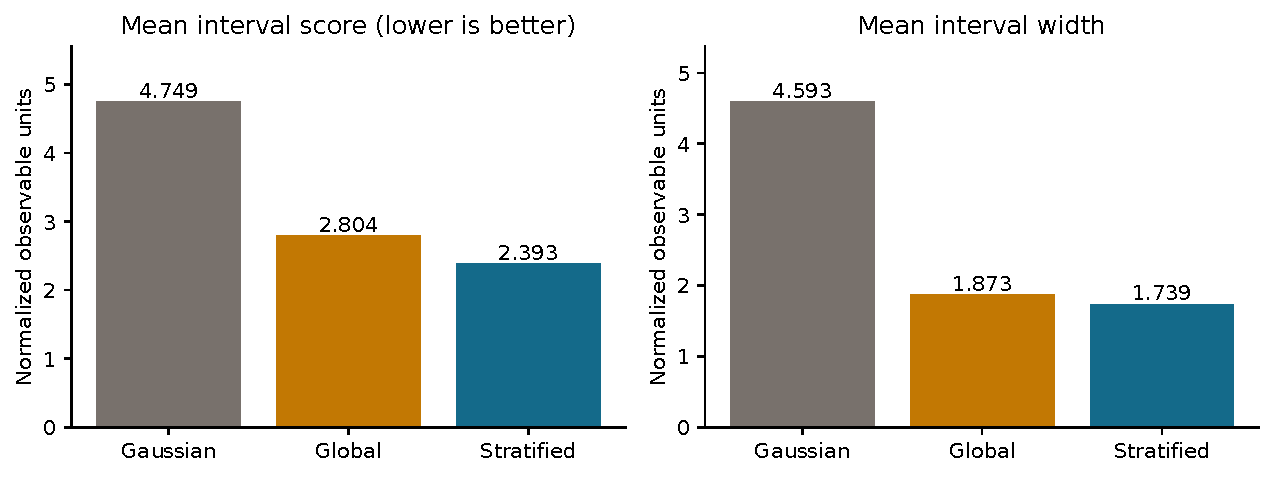
\includegraphics[width=\textwidth]{browser-interval-efficiency.pdf}
\caption{Mean interval score and width from all 800 independent confirmation
series. The three procedures share point forecasts; these plotted means do not
represent independently estimated confidence intervals.}
\label{fig:browser-efficiency}\end{figure}

Uncertainty is summarized by drawing 10,000 paired bootstrap samples of the
800 complete series with local PCG64 seed 20261108. Within a draw, the same
series indices are used for both interval procedures. Forecast leads are not
resampled as independent observations. The stratified-minus-Gaussian mean
interval-score difference is $-2.355627$, with exploratory 95\% percentile
interval $[-2.437258,-2.273077]$. The stratified-minus-global difference is
$-0.410424$, with interval $[-0.451789,-0.368795]$. These are unadjusted
exploratory intervals under the experiment's independent-series design, not
multiplicity-controlled evidence about every reported subgroup. Respectively,
778 and 606 of 800 series have strictly lower interval score, so the mean
advantage does not conceal a majority of series with larger losses.

\begin{figure}[htbp]\centering
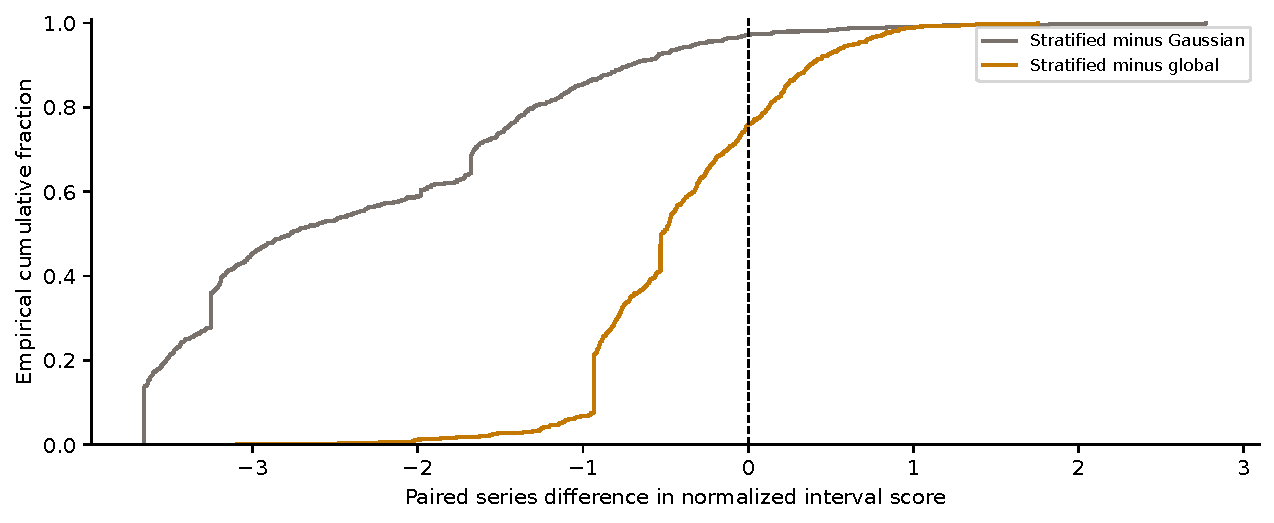
\includegraphics[width=\textwidth]{browser-paired-scores.pdf}
\caption{Empirical distributions of paired interval-score differences for
individual confirmation series. Negative values favor prefix stratification;
the positive tails retain series on which the comparison is unfavorable.}
\label{fig:browser-paired}\end{figure}

Figure~\ref{fig:browser-paired} makes the individual-loss distribution visible
alongside its aggregate uncertainty. Some prefixes benefit little and some
have larger interval penalties after stratification. No series is removed
because its interval score worsens. The empirical distribution is a description
of these 800 generated series; its tails cannot establish the frequency of
rare failures in an operational population absent from the generator.

\begin{table}[htbp]\centering
\caption{Prefix-bin calibration support and held-out coverage. Fixed bins use
observed histories alone; their coverage summaries do not guarantee validity
for every hidden generating mechanism or individual prefix.}
\label{tab:browser-groups}
\begin{tabular}{lrr}\toprule
Observed-prefix roughness & Calibration series & Test coverage\\\midrule
$[0,0.5)$ & 115 & 0.843377\\
$[0.5,1.25)$ & 120 & 0.804773\\
$[1.25,\infty)$ & 165 & 0.826786\\\bottomrule
\end{tabular}\end{table}

Table~\ref{tab:browser-groups} reports coverage in the observable bins targeted
by the stratified construction. Family-specific results remain distinct.
Coverage is 80.46\% for noise, 74.57\% for trend, 86.71\% for seasonality and
88.92\% for trend plus seasonality. Figure~\ref{fig:browser-families} shows
that stratification addresses the large noise-family shortfall of global
calibration without eliminating all family differences. In particular, the
trend family remains below nominal coverage. These family outcomes were not
used to redraw the bins after the confirmation was scored.

\begin{figure}[htbp]\centering
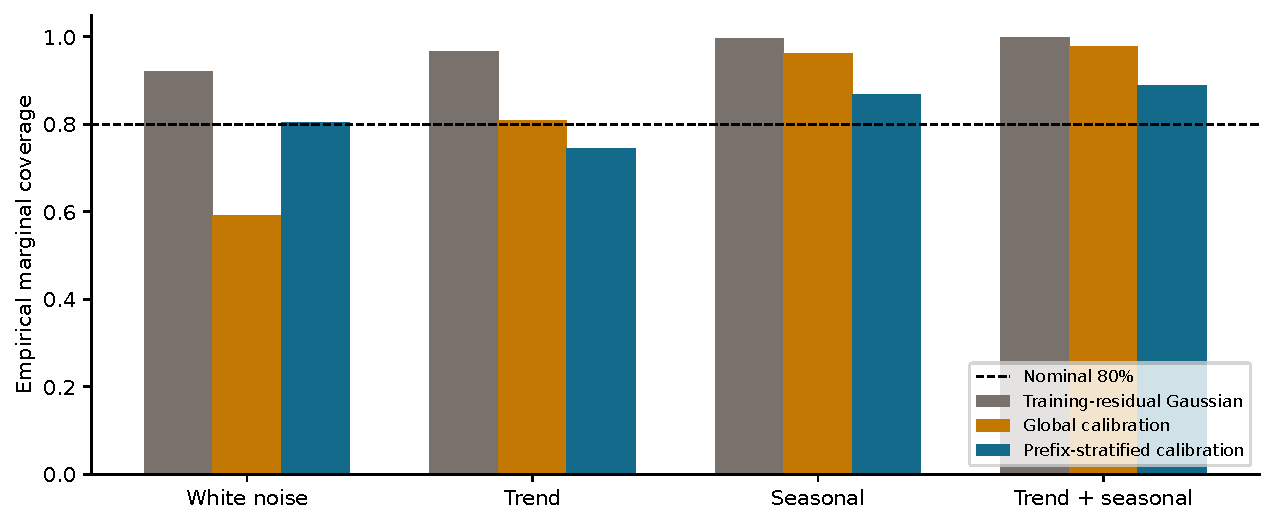
\includegraphics[width=\textwidth]{browser-family-coverage.pdf}
\caption{Confirmation coverage by latent generator family for identical point
forecasts. Prefix stratification improves the noise-family shortfall, while
the trend family's remaining undercoverage prevents a universal calibration claim.}
\label{fig:browser-families}\end{figure}

Figure~\ref{fig:browser-leads} shows lead-specific coverage, ranging from
79.50\% to 85.13\% for the stratified rule. Separate marginal radii allow
different error distributions at different leads. They do not force a
monotone square-root growth law and do not imply a joint prediction region.
The experiment's prospectively fixed engineering criteria require identical
point forecasts, adequate calibration support, lower mean interval score,
overall coverage between 75\% and 85\%, bin coverage between 70\% and 90\%,
and normalized runtime error below $10^{-4}$. All six passed. This admission
decision is explicitly weaker than demonstrating calibration on real data.

\begin{figure}[htbp]\centering
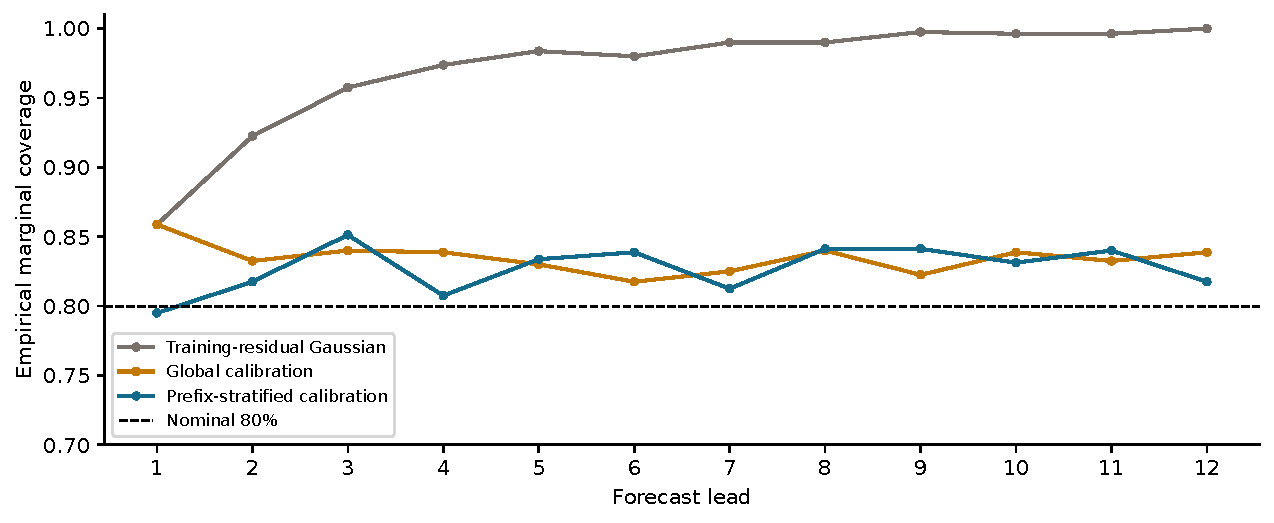
\includegraphics[width=\textwidth]{browser-lead-coverage.pdf}
\caption{Empirical coverage at each of twelve future leads. The dashed line
marks nominal marginal coverage; the graph does not report simultaneous
coverage of an entire forecast trajectory.}
\label{fig:browser-leads}\end{figure}

\subsection{Unit invariance, reproducibility and applicability}
\label{sec:browser-validation}

Consider a positive change of units and location, $x'_i=ax_i+b$, $a>0$.
Then $s(x')=as(x)$ and $z'_i=z_i$. The frozen matrix therefore returns the
same normalized point vector. Equation~\ref{eq:browser-inverse} gives
$\hat a'_h=a\hat a_h+b$. Both the numerator and denominator of
Equation~\ref{eq:browser-roughness} are multiplied by $a^2$, so the selected
bin is unchanged. The calibrated endpoints transform as
\begin{equation}
 I'_h(x')=aI_h(x)+b.
 \label{eq:browser-units}
\end{equation}
Normalized errors, widths and interval scores are consequently unchanged in
exact arithmetic. Float32 execution and finite-precision computation of the
observed scale introduce small numerical differences, which are tested with
explicit tolerances. This invariance explains why an observed-data scale is
required and why a fallback measured in arbitrary raw units is inadmissible.
It does not prove correctness of every other method in the product.

All 2,600 generated series across the two experiments are retained, together
with their full-sequence hashes and every test target, point prediction and
interval endpoint. The first experiment was executed in two separate processes
and every generated output byte matched. An independent checker imports no
training, calibration or scoring producer: it recomputes all stored losses,
prefix groups, partition disjointness and source bindings. Its runtime mode
also reconstructs every calibration radius and test prediction directly from
the stored graph weights and actual ONNX execution. The independently measured
maximum normalized arithmetic discrepancy is below $10^{-6}$.

These checks support an auditable computational conclusion: within the
specified synthetic mixture, the stratified interval rule improves interval
score around the preserved point forecast. They do not establish an advantage
for the discarded ridge point model, generalize the generator to authentic
industrial observations, or validate an action policy based on the bands.
Before such use, the relevant population, observation revisions, forecast
horizon, loss asymmetry and calibration/update schedule must be specified and
tested with independent data. The browser retains these limits in its
description instead of presenting the nominal level as an unconditional
promise for every uploaded series.
